\section{The identification of conduct}\label{sec:03-identification}

The tests of \cref{sec:03-sumner,sec:03-revenue-tests} move cost and watch prices. Cost shifters trace out the
demand curve, so they speak to the supply relation only indirectly, and they deliver tests or bounds. This section
asks the reverse question. What do movements in demand reveal about conduct? The answer, due to
\citet{Bresnahan1982} and \citet{Lau1982}, has two halves. When the slope of marginal cost is unknown, demand shifts
that move the demand curve in parallel reveal nothing about conduct. Shifts that change the slope of demand identify it. \Cref{sec:01-identification} previews the
argument. Here we develop the full theory. We cover the linear model and its observational equivalence, the rotation
argument and its estimation, a general version of Lau's theorem with proof, and the other routes used in practice.

\subsection{The linear model and observational equivalence}\label{sec:03-obs-equiv}

We start from the simplest model in which the question can be posed. It is the model of \citet{Bresnahan1982}, which
\citet[Section~3.1]{Bresnahan1989} uses to explain how the data identify market power. Markets are indexed by
$t = 1, \dots, T$, which may be periods, locations or both.

\begin{assumption}[Linear market]\label{ass:03-linear}
\leavevmode
\begin{enumerate}[label=(\roman*)]
\item Market demand is $Q_t = a_0 + a_1 P_t + a_2 Y_t + u^d_t$ with $a_1 < 0$ and $a_2 \neq 0$. The variable $Y_t$ is
  an observed \emph{demand shifter}.
\item Industry marginal cost is $MC_t = b_0 + b_1 Q_t + b_2 W_t + u^s_t$ with $b_2 \neq 0$. The variable $W_t$ is an
  observed \emph{cost shifter}.
\item Conduct is a constant $\theta \ge 0$. Perceived marginal revenue $P_t + \theta Q_t \frac{\partial P_t}{\partial
  Q_t}$ equals marginal cost.
\item The errors satisfy $\E[u^d_t \mid Y_t, W_t] = \E[u^s_t \mid Y_t, W_t] = 0$, and the vector $(1, Y_t, W_t)$ has a
  nonsingular second-moment matrix.
\end{enumerate}
\end{assumption}

Part (iii) is the supply relation \eqref{eq:03-supply-relation} with a linear demand curve. The slope of inverse demand
is $\frac{\partial P_t}{\partial Q_t} = \frac{1}{a_1}$, so perceived marginal revenue is $P_t + \theta\frac{Q_t}{a_1}$.
Setting it equal to marginal cost and solving for price gives
\begin{equation*}
P_t = MC_t - \theta\frac{Q_t}{a_1} = b_0 + b_1 Q_t + \theta\left(-\frac{Q_t}{a_1}\right) + b_2 W_t + u^s_t .
\end{equation*}
The term $-\theta\frac{Q_t}{a_1} = \theta\frac{Q_t}{\lvert a_1\rvert} \ge 0$ is the markup. Collecting the two terms in
$Q_t$, the model consists of three equations:
\begin{equation}\label{eq:03-linear-system}
\begin{aligned}
\text{demand:}\quad & Q_t = a_0 + a_1 P_t + a_2 Y_t + u^d_t ,\\
\text{marginal cost:}\quad & MC_t = b_0 + b_1 Q_t + b_2 W_t + u^s_t ,\\
\text{supply relation:}\quad & P_t = b_0 + \lambda Q_t + b_2 W_t + u^s_t, \qquad \lambda \equiv b_1 - \frac{\theta}{a_1} .
\end{aligned}
\end{equation}
The \emph{composite slope} $\lambda$ adds the slope of marginal cost, $b_1$, to the conduct-weighted magnitude of the
slope of inverse demand, $\frac{\theta}{\lvert a_1 \rvert}$. Only demand and the supply relation involve observed
endogenous variables, so the estimation problem has two equations.

\casehead{The reduced form}
Substituting the supply relation into demand gives
\begin{align*}
Q_t &= a_0 + a_1\left(b_0 + \lambda Q_t + b_2 W_t + u^s_t\right) + a_2 Y_t + u^d_t ,\\
(1 - a_1\lambda)\, Q_t &= a_0 + a_1 b_0 + a_2 Y_t + a_1 b_2 W_t + u^d_t + a_1 u^s_t .
\end{align*}
Let $\Delta \equiv 1 - a_1\lambda = 1 + \theta - a_1 b_1$. It is positive whenever $b_1 \ge 0$, because $a_1 < 0$, and we
assume $\Delta > 0$ throughout. Dividing by $\Delta$ and substituting back into the supply relation yields the reduced form
\begin{equation}\label{eq:03-linear-rf}
Q_t = \frac{a_0 + a_1 b_0 + a_2 Y_t + a_1 b_2 W_t + u^d_t + a_1 u^s_t}{\Delta}, \qquad
P_t = \frac{b_0 + \lambda a_0 + \lambda a_2 Y_t + b_2 W_t + \lambda u^d_t + u^s_t}{\Delta}.
\end{equation}
The reduced-form coefficients on the shifters are $\pi_{QY} = \frac{a_2}{\Delta}$, $\pi_{PY} = \frac{\lambda a_2}{\Delta}$,
$\pi_{QW} = \frac{a_1 b_2}{\Delta}$ and $\pi_{PW} = \frac{b_2}{\Delta}$. Regressions of $P_t$ and $Q_t$ on $(1, Y_t, W_t)$
identify all four. Two ratios then deliver the slopes:
\begin{equation*}
a_1 = \frac{\pi_{QW}}{\pi_{PW}}, \qquad \lambda = \frac{\pi_{PY}}{\pi_{QY}} .
\end{equation*}
A cost shift moves the equilibrium along the demand curve, so the ratio of the quantity response to the price response
is the slope of demand. A demand shift moves the equilibrium along the supply relation, so the ratio of the price
response to the quantity response is the slope of the supply relation. With $\Delta = 1 - a_1\lambda$ in hand,
$a_2 = \Delta\pi_{QY}$ and $b_2 = \Delta\pi_{PW}$, and the intercepts follow. Each equation is exactly identified, so this
indirect least squares solution coincides with two-stage least squares (2SLS). Demand is estimated by 2SLS of $Q_t$ on
$(1, P_t, Y_t)$ with instruments $(1, Y_t, W_t)$. The supply relation is estimated by 2SLS of $P_t$ on $(1, Q_t, W_t)$
with the same instruments (\cref{app:econometrics}).

\begin{proposition}[Observational equivalence]\label{prop:03-obs-equiv}
Let the structure $(a_0, a_1, a_2, b_0, b_1, b_2, \theta)$ and the distribution of $(u^d_t, u^s_t)$ satisfy
\cref{ass:03-linear} with $\Delta > 0$. For any $\theta' \ge 0$, replace $(b_1, \theta)$ by $(b_1', \theta')$ with
\begin{equation*}
b_1' = b_1 + \frac{\theta' - \theta}{a_1},
\end{equation*}
and keep everything else. The new structure generates the same conditional distribution of $(P_t, Q_t)$ given
$(Y_t, W_t)$. Hence $\theta$ and $b_1$ are not separately identified.
\end{proposition}

\begin{proof}
The composite slope of the new structure is
\begin{equation*}
\lambda' = b_1' - \frac{\theta'}{a_1} = b_1 + \frac{\theta' - \theta}{a_1} - \frac{\theta'}{a_1} = b_1 - \frac{\theta}{a_1}
= \lambda ,
\end{equation*}
and therefore $\Delta' = 1 - a_1\lambda' = \Delta > 0$. The reduced form \eqref{eq:03-linear-rf} depends on the structure
only through $(a_0, a_1, a_2, b_0, \lambda, b_2)$ and the errors, and none of these has changed. The two structures map
every value of $(Y_t, W_t, u^d_t, u^s_t)$ into the same $(P_t, Q_t)$, so the conditional distributions coincide.
\end{proof}

The set of structures that fit the data is the line $b_1 = \lambda + \frac{\theta}{a_1}$ in the $(\theta, b_1)$ plane. It
slopes down because $a_1 < 0$. More market power must be offset by flatter marginal cost. A sign restriction on the
slope of marginal cost turns this line into an interval for conduct.

\begin{corollary}[An interval for conduct]\label{cor:03-obs-equiv-bounds}
Under \cref{ass:03-linear}, suppose $\lambda > 0$ and marginal cost does not fall with output, $b_1 \ge 0$. Then the
values of conduct consistent with the data form the interval $\theta \in [0, \lvert a_1\rvert\lambda]$. Constant marginal
cost ($b_1 = 0$) selects the upper endpoint, and price taking selects the lower endpoint. If $\lvert a_1\rvert\lambda < 1$,
the data reject monopoly with nondecreasing marginal cost.
\end{corollary}

\begin{proof}
By \cref{prop:03-obs-equiv}, every pair $(\theta, \lambda + \frac{\theta}{a_1})$ with $\theta \ge 0$ fits the data. The
restriction $b_1 \ge 0$ reads $\lambda + \frac{\theta}{a_1} \ge 0$. Multiplying by $a_1 < 0$ reverses the inequality and gives
$a_1\lambda + \theta \le 0$, that is, $\theta \le -a_1\lambda = \lvert a_1\rvert\lambda$. Together with $\theta \ge 0$ this
is the interval. Monopoly, $\theta = 1$, lies in it exactly when $1 \le \lvert a_1\rvert\lambda$.
\end{proof}

The interval is the demand-side counterpart of the cost-side bounds of \cref{sec:03-sullivan}. It also shows what the
assumption of constant marginal cost buys. It picks the largest conduct consistent with the data, because it attributes
the entire slope of the supply relation to market power.

\casehead{A graphical version}
\Cref{fig:03-bresnahan-shift} redraws Figure~1 of \citet{Bresnahan1982}, a schematic, with illustrative numbers of
our own. Inverse demand shifts from
$D_1\colon P = 10 - Q$ to $D_2\colon P = 12 - Q$, so $a_1 = -1$ in both markets. The competitive model has marginal cost
$MC^c = 2 + 1.1Q$ and $\theta = 0$. The monopoly model has $MC^m = 2 + 0.1Q$ and $\theta = 1$. Both have composite slope
$\lambda = 1.1$. Under competition the first equilibrium solves $10 - Q = 2 + 1.1Q$, so $Q = \frac{8}{2.1} = 3.81$ and
$P = 6.19$. Under monopoly, marginal revenue $MR_1 = 10 - 2Q$ equals $MC^m$ where $10 - 2Q = 2 + 0.1Q$. This gives the
same quantity $\frac{8}{2.1}$ and, reading price off demand, the same price. After the shift both models predict
$Q = \frac{10}{2.1} = 4.76$ and $P = 7.24$. The two models produce the equilibria $E_1$ and $E_2$ exactly.

\begin{figure}[htbp]
\centering
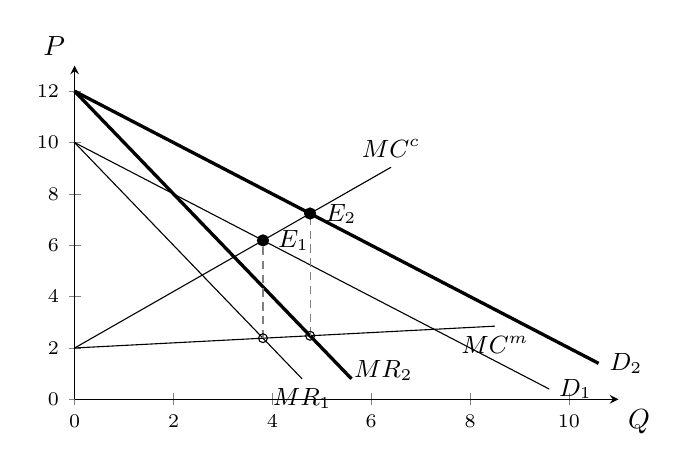
\begin{tikzpicture}
\begin{axis}[
  width=0.70\textwidth, height=0.48\textwidth,
  xmin=0, xmax=11, ymin=0, ymax=13,
  axis lines=left, xlabel={$Q$}, ylabel={$P$},
  xtick={0,2,4,6,8,10}, ytick={0,2,4,6,8,10,12},
  tick label style={font=\scriptsize},
  every axis x label/.style={at={(ticklabel* cs:1)}, anchor=north west},
  every axis y label/.style={at={(ticklabel* cs:1)}, anchor=south east},
  clip=false]
  \addplot[thin, domain=0:9.6, samples=2] {10 - x} node[pos=1, right, font=\small] {$D_1$};
  \addplot[very thick, domain=0:10.6, samples=2] {12 - x} node[pos=1, right, font=\small] {$D_2$};
  \addplot[thin, domain=0:4.6, samples=2] {10 - 2*x} node[pos=1, below, font=\small] {$MR_1$};
  \addplot[very thick, domain=0:5.6, samples=2] {12 - 2*x} node[pos=0.97, anchor=west, font=\small] {$MR_2$};
  \addplot[thin, domain=0:6.4, samples=2] {2 + 1.1*x} node[pos=1, above, font=\small] {$MC^c$};
  \addplot[thin, domain=0:8.5, samples=2] {2 + 0.1*x} node[pos=1, below, font=\small] {$MC^m$};
  \draw[densely dashed, gray] (axis cs:3.8095,2.381) -- (axis cs:3.8095,6.1905);
  \draw[densely dashed, gray] (axis cs:4.7619,2.476) -- (axis cs:4.7619,7.2381);
  \addplot[only marks, mark=*, mark size=2pt] coordinates {(3.8095,6.1905) (4.7619,7.2381)};
  \addplot[only marks, mark=o, mark size=1.6pt] coordinates {(3.8095,2.381) (4.7619,2.476)};
  \node[right, font=\small] at (axis cs:3.92,6.2) {$E_1$};
  \node[right, font=\small] at (axis cs:4.88,7.22) {$E_2$};
\end{axis}
\end{tikzpicture}
\caption[Observational equivalence under a parallel demand shift]{Observational equivalence under a parallel demand
shift. Demand shifts from $D_1\colon P = 10 - Q$ to $D_2\colon P = 12 - Q$. Competitive firms with $MC^c = 2 + 1.1Q$ and a
monopolist with $MC^m = 2 + 0.1Q$ both produce $E_1 = (3.81, 6.19)$ and $E_2 = (4.76, 7.24)$. Under monopoly, output is
set where $MR_i$ crosses $MC^m$ (open circles) and price is read off demand (dashed lines). Drawn after Figure~1 of
\citet{Bresnahan1982}, with illustrative numbers chosen here.}
\label{fig:03-bresnahan-shift}
\end{figure}

The two readings of the same data differ greatly in what they say about welfare. In the competitive reading the Lerner
index at $E_1$ is zero. In the monopoly reading marginal cost at $E_1$ is $2 + 0.1 \times 3.81 = 2.38$, so the Lerner
index is $\frac{6.19 - 2.38}{6.19} = 0.62$. The economics behind the equivalence is simple. When demand shifts out, price
rises in both models. Under competition it rises because marginal cost rises steeply with output. Under monopoly it rises
because marginal revenue shifts out while marginal cost barely moves. A parallel shift raises price either because
marginal cost rises with output or because of market power, and the ratio $\frac{\Delta P}{\Delta Q} = \lambda$ is the
same in both cases.

\subsection{Rotations of demand identify conduct}\label{sec:03-rotation}

\citet{Bresnahan1982} breaks the equivalence by letting an exogenous variable change the slope of demand. Let $Z_t$ be an
observed \emph{demand rotator}, and write demand as
\begin{equation}\label{eq:03-rotation-demand}
Q_t = a_0 + a_1 P_t + a_2 Y_t + a_3 P_t Z_t + a_4 Z_t + u^d_t ,
\end{equation}
with $a_1 + a_3 Z_t < 0$ on the support of $Z_t$. The slope of demand is $\frac{\partial Q_t}{\partial P_t} = a_1 + a_3 Z_t$,
which varies with $Z_t$ when $a_3 \neq 0$. We let $Z_t$ also shift the level of demand through $a_4$. Nothing below
requires $a_4 = 0$. Perceived marginal revenue is now $P_t + \theta\frac{Q_t}{a_1 + a_3 Z_t}$, and the supply relation
becomes
\begin{equation}\label{eq:03-rotation-supply}
P_t = b_0 + b_1 Q_t + \theta Q^*_t + b_2 W_t + u^s_t, \qquad
Q^*_t \equiv -\frac{Q_t}{a_1 + a_3 Z_t} = \frac{Q_t}{\lvert a_1 + a_3 Z_t\rvert} .
\end{equation}
The variable $Q^*_t$ is the \emph{markup term} $m_t \equiv \frac{Q_t}{\left\lvert \frac{\partial Q_t}{\partial P_t}\right\rvert} =
\frac{P_t}{\varepsilon_t}$. It is the dollar markup a monopolist would charge, so $\theta Q^*_t$ is the markup. With
$a_3 = 0$ the markup term is proportional to $Q_t$, and \eqref{eq:03-rotation-supply} collapses to the supply relation of
\eqref{eq:03-linear-system}. With $a_3 \neq 0$, the markup term moves with $Z_t$ at a given quantity, while the cost term
$b_1 Q_t$ does not.

\begin{proposition}[Rotations identify conduct]\label{prop:03-rotation}
Let demand be \eqref{eq:03-rotation-demand} with known parameters, and let the supply relation be
\eqref{eq:03-rotation-supply}. Let $X_t = (Y_t, Z_t, W_t)$, assume $\E[u^s_t \mid X_t] = 0$, and assume $Z_t$ does not
enter marginal cost. Suppose $\mu(X_t) \equiv \E[Q_t \mid X_t]$ is strictly monotone in $Y_t$ for each $(Z_t, W_t)$,
$a_3 \neq 0$, $Z_t$ takes at least two values, and $W_t$ is not degenerate. Then $(b_0, b_1, b_2, \theta)$ are identified.
\end{proposition}

\begin{proof}
Write $Q^*_t = g(Z_t)Q_t$ with $g(Z) \equiv -\frac{1}{a_1 + a_3 Z}$, a known function. Taking expectations of
\eqref{eq:03-rotation-supply} conditional on $X_t$ gives
\begin{equation*}
\E[P_t \mid X_t] = b_0 + b_1\, \mu(X_t) + \theta\, g(Z_t)\, \mu(X_t) + b_2 W_t .
\end{equation*}
The left side and $\mu(X_t)$ are features of the distribution of the data. Suppose a second vector $(b_0', b_1', b_2',
\theta')$ satisfies the same equation. Subtracting, the differences $c = (b_0 - b_0', b_1 - b_1', b_2 - b_2', \theta -
\theta')$ satisfy
\begin{equation*}
0 = c_0 + c_1\, \mu(X) + c_3\, g(Z)\, \mu(X) + c_2 W \quad \text{for all } X .
\end{equation*}
Fix $(Z, W)$ and vary $Y$. Since $\mu$ changes with $Y$, the coefficient on $\mu$ must vanish: $c_1 + c_3 g(Z) = 0$ for
every $Z$. Because $a_3 \neq 0$, the function $g$ takes different values at two values of $Z$, so $c_1 = c_3 = 0$. The
remaining condition $c_0 + c_2 W = 0$ for all $W$ gives $c_0 = c_2 = 0$.
\end{proof}

The proof has a transparent deterministic core. Suppose two markets share the same $W$ and the same quantity $Q$ but have
different rotators $Z_1 \neq Z_2$. The demand shifter $Y$ can always be chosen to make this happen. Marginal cost is then
the same in both markets, and the price difference isolates the markup:
\begin{equation*}
P_1 - P_2 = \theta\, Q\left[g(Z_1) - g(Z_2)\right] .
\end{equation*}
The bracket is nonzero when $a_3 \neq 0$, so the price difference reveals $\theta$. Once $\theta$ is known, two markets
with the same $Z$ and different $Q$ reveal $b_1$.

\casehead{Estimation}
The natural estimator has two steps. In the first step we estimate demand \eqref{eq:03-rotation-demand} by 2SLS. The
regressors $P_t$ and $P_tZ_t$ are endogenous, $(1, Y_t, Z_t)$ are included exogenous variables, and $W_t$ and $W_tZ_t$
are the excluded instruments. In the second step we construct
\begin{equation*}
\hat Q^*_t = -\frac{Q_t}{\hat a_1 + \hat a_3 Z_t}
\end{equation*}
and estimate the supply relation $P_t = b_0 + b_1 Q_t + \theta \hat Q^*_t + b_2 W_t + e_t$ by 2SLS. Here $Q_t$ and
$\hat Q^*_t$ are endogenous, $(1, W_t)$ are included exogenous variables, and $(Y_t, Z_t, Y_tZ_t)$ are the excluded
instruments. Three instruments for two endogenous regressors leave one overidentifying restriction to test. Because
$\hat Q^*_t$ is a generated regressor, conventional second-step standard errors are too small.
\citet[p.~1033, fn.~23]{Bresnahan1989} calls this explicit two-step procedure ``so ugly that no one would ever undertake
it'', while noting that it shows why more powerful techniques identify $\theta$.

The better procedure estimates both equations jointly by the generalized method of moments (GMM). Stack the parameters in
$\Theta = (a_0, \dots, a_4, b_0, b_1, b_2, \theta)$ and define the residuals
\begin{equation}\label{eq:03-rotation-gmm}
\begin{aligned}
u^d_t(\Theta) &= Q_t - a_0 - a_1 P_t - a_2 Y_t - a_3 P_t Z_t - a_4 Z_t ,\\
u^s_t(\Theta) &= P_t - b_0 - b_1 Q_t + \theta\, \frac{Q_t}{a_1 + a_3 Z_t} - b_2 W_t .
\end{aligned}
\end{equation}
With instrument vectors $h^d_t = (1, Y_t, Z_t, W_t, W_tZ_t)^\top$ and $h^s_t = (1, W_t, Y_t, Z_t, Y_tZ_t)^\top$, the
moment conditions are $\E[h^d_t u^d_t(\Theta)] = 0$ and $\E[h^s_t u^s_t(\Theta)] = 0$. GMM minimizes a quadratic form in the
sample analogues of the ten moments. The system is nonlinear in $\Theta$ because $\theta$ multiplies a ratio that involves
$(a_1, a_3)$. Joint estimation imposes the cross-equation restriction that the slope inside the markup term equals the
slope of demand, and its standard errors account for the estimation of demand automatically (\cref{app:econometrics}).

\casehead{A graphical version}
\Cref{fig:03-bresnahan-rotation} redraws Figure~2 of \citet{Bresnahan1982} in the same way. We keep $D_1$, $MC^c$, $MC^m$ and
$E_1 = (3.81, 6.19)$ from \cref{fig:03-bresnahan-shift}. Demand rotates around $E_1$ to the flatter curve
$D_3\colon P = 7.714 - 0.4Q$, which passes through $E_1$ because $6.19 + 0.4 \times 3.81 = 7.714$. The competitive
equilibrium solves $7.714 - 0.4Q = 2 + 1.1Q$, so $Q = \frac{5.714}{1.5} = 3.81$. Competition stays at $E_1$. The monopolist
sets $MR_3 = 7.714 - 0.8Q$ equal to $2 + 0.1Q$, so $Q = \frac{5.714}{0.9} = 6.35$ and $P = 7.714 - 0.4 \times 6.35 = 5.17$.
Monopoly moves to $E_3 = (6.35, 5.17)$. At $E_1$ the elasticity of demand rises from $\frac{6.19}{3.81} = 1.62$ to
$\frac{6.19}{0.4 \times 3.81} = 4.06$, and the monopolist cuts its markup.

\begin{figure}[htbp]
\centering
\begin{tikzpicture}
\begin{axis}[
  width=0.70\textwidth, height=0.45\textwidth,
  xmin=0, xmax=11, ymin=0, ymax=10.8,
  axis lines=left, xlabel={$Q$}, ylabel={$P$},
  xtick={0,2,4,6,8,10}, ytick={0,2,4,6,8,10},
  tick label style={font=\scriptsize},
  every axis x label/.style={at={(ticklabel* cs:1)}, anchor=north west},
  every axis y label/.style={at={(ticklabel* cs:1)}, anchor=south east},
  clip=false]
  \addplot[thin, domain=0:9.3, samples=2] {10 - x} node[pos=1, right, font=\small] {$D_1$};
  \addplot[thin, domain=0:4.6, samples=2] {10 - 2*x} node[pos=1, below, font=\small] {$MR_1$};
  \addplot[very thick, domain=0:10.6, samples=2] {7.7143 - 0.4*x} node[pos=1, right, font=\small] {$D_3$};
  \addplot[very thick, domain=0:8.6, samples=2] {7.7143 - 0.8*x} node[pos=1, below, font=\small] {$MR_3$};
  \addplot[thin, domain=0:6.4, samples=2] {2 + 1.1*x} node[pos=1, above, font=\small] {$MC^c$};
  \addplot[thin, domain=0:9.2, samples=2] {2 + 0.1*x} node[pos=1, right, font=\small] {$MC^m$};
  \draw[densely dashed, gray] (axis cs:6.3492,2.635) -- (axis cs:6.3492,5.1746);
  \addplot[only marks, mark=*, mark size=2.2pt] coordinates {(3.8095,6.1905)};
  \addplot[only marks, mark=*, mark size=1.6pt] coordinates {(6.3492,5.1746)};
  \addplot[only marks, mark=o, mark size=1.6pt] coordinates {(3.8095,2.381) (6.3492,2.635)};
  \node[font=\small] (e1lab) at (axis cs:3.2,7.7) {$E_1$};
  \draw[->, >=Stealth, thin] (e1lab.south east) -- (axis cs:3.74,6.33);
  \node[above right, font=\small] at (axis cs:6.35,5.25) {$E_3$};
\end{axis}
\end{tikzpicture}
\caption[A demand rotation separates competition from monopoly]{A demand rotation separates competition from monopoly.
Demand rotates around $E_1 = (3.81, 6.19)$ from $D_1\colon P = 10 - Q$ to $D_3\colon P = 7.714 - 0.4Q$. Competitive firms
with $MC^c = 2 + 1.1Q$ stay at $E_1$. A monopolist with $MC^m = 2 + 0.1Q$ sets $MR_3 = MC^m$ (open circle) and moves to
$E_3 = (6.35, 5.17)$. Drawn after Figure~2 of \citet{Bresnahan1982}, with illustrative numbers chosen here.}
\label{fig:03-bresnahan-rotation}
\end{figure}

The rotation does more than separate two polar models. The size of the response measures conduct. Write the magnitudes of
the inverse-demand slopes before and after the rotation as $g_1 = g(Z_1)$ and $g_3 = g(Z_3)$, with the function
$g(Z) = -\frac{1}{a_1 + a_3 Z} = \frac{1}{\lvert a_1 + a_3 Z\rvert}$ from the proof of \cref{prop:03-rotation}.
Every structure consistent with the original market has marginal cost slope $b_1(\theta) = \lambda_1 - \theta g_1$, where
$\lambda_1$ is the composite slope estimated before the rotation. After the rotation the supply relation has slope
$b_1(\theta) + \theta g_3 = \lambda_1 - \theta(g_1 - g_3)$. Since the original supply relation passed through $(Q_1, P_1)$,
the new one is
\begin{equation*}
P = P_1 + \left[\lambda_1 - \theta(g_1 - g_3)\right](Q - Q_1) - \theta(g_1 - g_3) Q_1 .
\end{equation*}
The rotated demand curve is $P = P_1 - g_3(Q - Q_1)$. Equating the two and solving,
\begin{align*}
(Q - Q_1)\left[g_3 + \lambda_1 - \theta(g_1 - g_3)\right] &= \theta(g_1 - g_3) Q_1 ,\\
Q_3 - Q_1 &= \frac{\theta(g_1 - g_3)Q_1}{g_3 + \lambda_1 - \theta(g_1 - g_3)} .
\end{align*}
Rearranging the first line at $Q = Q_3$ expresses conduct in terms of observables:
\begin{equation}\label{eq:03-rotation-response}
\theta = \frac{(g_3 + \lambda_1)(Q_3 - Q_1)}{(g_1 - g_3)\, Q_3} .
\end{equation}
In the example $g_1 = 1$, $g_3 = 0.4$ and $\lambda_1 = 1.1$. The response is zero under competition, $2.54$ under
monopoly, and $0.95$ when $\theta = 0.5$. Plugging the monopoly outcome into \eqref{eq:03-rotation-response} gives
$\frac{1.5 \times 2.54}{0.6 \times 6.35} = 1.00$. When demand becomes more elastic, a firm with market power cuts its
markup, and its output response rises with its conduct. At the original quantity the supply relation shifts down by
$\theta(g_1 - g_3)Q_1$, an amount proportional to conduct.

\casehead{Rotators in practice}
Applications need a natural experiment that changes the slope of demand \citep[pp.~1033--1034]{Bresnahan1989}. One
shifter might measure the size of the economy, such as national income, while a second measures the price of a
substitute. In \citet{JustChern1980} the market power lies on the buying side. Tomato processors buy from many farmers,
and the adoption of a mechanical harvester changed the elasticity of supply they faced. In
\citet{Bresnahan1981,Bresnahan1987} demand elasticities depend on how crowded the product space is, which changes with
the set of models offered (\cref{ch:discrete}). In sugar refining the canning season changes the composition of buyers
and makes demand less elastic (\cref{sec:03-sugar}). The method stands or falls with the estimated demand elasticities.
Critics offered other readings of the tomato harvester, and the automobile results depend on how products are ordered in
quality space \citep[p.~1034]{Bresnahan1989}.

Two caveats follow from the theory. First, the rotator must be excluded from marginal cost. If the canning season also
changes the slope of marginal cost, through overtime for example, then a term $b_3 Z_t Q_t$ in marginal cost competes with
$\theta g(Z_t) Q_t$. The two differ only through the curvature of $g$, a thin reed for identification. Second, the
linear model can identify $\theta$ even without a separate shifter $Y_t$, using $Z_t$ and $Z_t^2$ as instruments. That
identification comes entirely from the linearity of marginal cost in quantity, as the next theorem shows.

\subsection{Lau's theorem: identification without functional forms}\label{sec:03-lau}

The rotation argument does not depend on linearity. \citet{Lau1982} shows that it holds for general demand and cost
functions. \citet[p.~1033]{Bresnahan1989} summarizes his sufficient condition for identification. The inverse demand
function must not be writable with the demand shifters separable from quantity, which requires at least two shifters.
We state and prove a version of this result.

Let inverse demand be $P = f(Q, Y)$ with a vector of demand shifters $Y \in \R^k$ and $f_Q < 0$, and let industry
marginal cost be an unknown function $c(Q, W)$. The supply relation is
\begin{equation}\label{eq:03-lau-model}
P = c(Q, W) - \theta\, Q\, f_Q(Q, Y) .
\end{equation}
Following Lau, we work without econometric errors. The data are the equilibrium map $(Y, W) \mapsto (P, Q)$.
\citet[p.~1776]{BerryHaile2014} describe the class Lau studied as deterministic conjectural-variations models with
homogeneous goods and symmetric firms. We make three assumptions. The demand function $f$ is known, because the cost
shifters $W$ are excluded from demand and trace it out. Each structure considered has a unique equilibrium with $Q > 0$
for every $(Y, W)$. The function $f$ is twice continuously differentiable.

\begin{definition}[Single-index demand]\label{def:03-single-index}
Inverse demand has a \emph{single index} if $f(Q, Y) = \tilde g(Q, r(Y))$ for a scalar function $r$ and some
function $\tilde g$.
\end{definition}

\begin{theorem}[Lau]\label{prop:03-lau}
\leavevmode
\begin{enumerate}[label=(\roman*)]
\item Suppose demand has a single index, and for each $W$ the equilibrium quantity $Q^e(r, W)$ is strictly monotone in
  the index $r$. Then for every $\theta' \ge 0$ there is a marginal cost function $c'(Q, W)$ such that the structure
  $(f, c', \theta')$ reproduces every observed equilibrium. Conduct is not identified.
\item Suppose that at some observed equilibrium $(Q_0, Y_0, W_0)$ the $2 \times k$ Jacobian of
  $\left(f(Q_0, Y), f_Q(Q_0, Y)\right)$ with respect to $Y$ has rank two at $Y_0$. Suppose also that the equilibrium
  map is observed for all $Y$ in a neighborhood of $Y_0$ with $W = W_0$. Then $\theta$ is identified.
\end{enumerate}
\end{theorem}

\begin{proof}
(i) Fix $W$. Because $Q^e(\cdot, W)$ is strictly monotone, it has an inverse $r = H(Q, W)$ on its range. Define
\begin{equation*}
c'(Q, W) \equiv \tilde g\left(Q, H(Q, W)\right) + \theta'\, Q\, \tilde g_Q\left(Q, H(Q, W)\right) ,
\end{equation*}
which depends on $(Q, W)$ only. Take any observed equilibrium $(P, Q)$ at $(Y, W)$ and let $r = r(Y)$. Then
$Q = Q^e(r, W)$, so $H(Q, W) = r$ and $P = \tilde g(Q, r)$. Substituting,
\begin{equation*}
c'(Q, W) = P + \theta'\, Q\, \tilde g_Q(Q, r) = P + \theta'\, Q\, f_Q(Q, Y) .
\end{equation*}
Rearranging gives $P = c'(Q, W) - \theta' Q f_Q(Q, Y)$, which is the supply relation of the alternative structure. Demand
is unchanged. The observed point is therefore an equilibrium of $(f, c', \theta')$, and by uniqueness it is the only one.

(ii) Fix $W_0$ and define $\Phi(Q, Y) \equiv f(Q, Y) + \theta Q f_Q(Q, Y) - c(Q, W_0)$, so equilibria satisfy
$\Phi = 0$. Consider the set $\Gamma = \{Y : \Phi(Q_0, Y) = 0\}$ of shifter values that produce the equilibrium quantity
$Q_0$. Its gradient at $Y_0$ is $\nabla f + \theta Q_0 \nabla f_Q$, where gradients are taken with respect to $Y$. This
gradient is nonzero, because $\nabla f$ and $\nabla f_Q$ are linearly independent. By the implicit function theorem,
$\Gamma$ is locally a manifold of dimension $k - 1$ through $Y_0$, with tangent space
$T = \{v : (\nabla f + \theta Q_0 \nabla f_Q)\cdot v = 0\}$. Suppose $f_Q(Q_0, \cdot)$ were constant on $\Gamma$ near
$Y_0$. Then $\nabla f_Q \cdot v = 0$ for all $v \in T$, so $\nabla f_Q = \ell(\nabla f + \theta Q_0\nabla f_Q)$ for some
scalar $\ell$. If $\ell \ne 0$, this makes $\nabla f$ and $\nabla f_Q$ linearly dependent. If $\ell = 0$, it makes
$\nabla f_Q = 0$. Both contradict rank two. Hence some $Y_1 \in \Gamma$ has $f_Q(Q_0, Y_1) \neq f_Q(Q_0, Y_0)$. The two
equilibria share $Q_0$ and $W_0$, hence the same marginal cost $c(Q_0, W_0)$. Subtracting their supply relations,
\begin{equation}\label{eq:03-lau-theta}
P_1 - P_0 = -\theta\, Q_0 \left[f_Q(Q_0, Y_1) - f_Q(Q_0, Y_0)\right], \qquad
\theta = -\frac{P_1 - P_0}{Q_0\left[f_Q(Q_0, Y_1) - f_Q(Q_0, Y_0)\right]} .
\end{equation}
Every term on the right is observed or known, so $\theta$ is identified.
\end{proof}

The two parts fit together. Under a single index, $f$ and $f_Q$ depend on $Y$ only through $r$. Their Jacobian is
$\left(\tilde g_r \nabla r, \tilde g_{Qr}\nabla r\right)$, which has rank at most one. Part (ii) is therefore the local
failure of the single-index structure. In words, $\theta$ is identified when the demand shifters can move the slope of
demand at a given quantity independently of its level. In the data, every observation with the same $W$ lies on a single
curve $P = \phi(Q, W)$ when demand has a single index. Any conduct value can then be rationalized by a suitable marginal
cost, as part (i) constructs.

Three examples make the condition concrete. Constant-elasticity demand with a scale shifter, $Q = Y P^{-\varepsilon}$, has
inverse demand $P = (\frac{Q}{Y})^{-\frac{1}{\varepsilon}}$, a single index. Conduct is not identified without restrictions
on cost. Letting a second shifter move the elasticity, $Q = Y_1 P^{-\varepsilon(Y_2)}$, breaks the single index. In the
linear rotation model \eqref{eq:03-rotation-demand}, inverse demand is $f = \frac{Q - a_0 - a_2 Y - a_4 Z}{a_1 + a_3 Z}$ with
$f_Q = \frac{1}{a_1 + a_3 Z}$. The Jacobian with respect to $(Y, Z)$ has determinant
\begin{equation*}
\frac{\partial f}{\partial Y}\frac{\partial f_Q}{\partial Z} - \frac{\partial f}{\partial Z}\frac{\partial f_Q}{\partial Y}
= \left(-\frac{a_2}{a_1 + a_3 Z}\right)\left(-\frac{a_3}{(a_1 + a_3 Z)^2}\right) - 0
= \frac{a_2 a_3}{(a_1 + a_3 Z)^3} ,
\end{equation*}
which is nonzero exactly when both $a_2 \neq 0$ and $a_3 \neq 0$. A pure rotator without a shifter ($a_2 = 0$) leaves a
single index $r = Z$, so the identification in the linear model with $a_2 = 0$ rests on the functional form of cost. This
matches an observation of \citet[p.~1754]{BerryHaile2014}. Lau's results require exogenous variation that alters both
the level and the slope of aggregate demand, a point they credit to \citet{Nevo1998}. Nothing in the proof uses
linearity, which is the sense in which the rotation argument is nonparametric.

\subsection{Other routes to identification}\label{sec:03-other-routes}

Demand rotations are one of several ways to separate conduct from the slope of marginal cost. Each replaces the rotator
with a restriction or with extra data, and each restriction has a cost.

Constant marginal cost makes a single demand shifter enough. With $b_1 = 0$ the composite slope is $\lambda =
-\frac{\theta}{a_1}$, so $\theta = -a_1\lambda$, the upper endpoint in \cref{cor:03-obs-equiv-bounds}. Equivalently,
pass-through reveals conduct. With linear demand and constant marginal cost, $\rho = \frac{1}{1 + \theta}$ by
\cref{cor:03-passthrough-cases}(iii), which is the logic of the pass-through tests of \cref{sec:03-passthrough-theory}.
The weakness is that any slope of marginal cost is read as market power, so the method overstates $\theta$ when
$b_1 > 0$.

Observed marginal cost removes the problem. Once demand is estimated, $\theta_t = \varepsilon_t L_t$ can be computed
observation by observation from \eqref{eq:03-lerner-theta}. This is the strategy of the two validation studies of this
chapter. In British electricity, marginal cost comes from fuel prices and plant efficiencies (\cref{sec:03-electricity}).
In insurance markets, claims data can play the same role, because the cost of serving a customer is the expected claim.
A related route assumes that cost is known up to a few parameters. In sugar refining the fixed-proportions technology
gives $MC = c_0 + kP^{raw}$, and $c_0$ and $k$ can be estimated jointly with $\theta$ or set from engineering evidence
(\cref{sec:03-sugar}).

Homogeneity of marginal cost in factor prices gives another restriction. Any term of the supply relation that does not
scale with factor prices must belong to the markup, the route of \citet{Appelbaum1982} described in
\cref{sec:03-taxonomy}. Firm-specific cost shifters identify a single firm's residual demand, an object different from
industry conduct (\cref{sec:03-residual-demand}).

Changes in market structure or regulation can shift conduct while leaving cost unchanged. \citet{SpillerFavaro1984} study
Uruguayan banking across a change in the regulation of entry. They find that freer entry shifts the supply relation
downward \citep[fn.~36]{Bresnahan1989}. The identifying assumption is that the regulatory change moved conduct and left
marginal cost alone.

Supply shocks identify regimes of conduct. \citet{Porter1983} lets the supply relation switch between a price-war regime
with low conduct and a collusive regime with high conduct. \citet[Section~3.4]{Bresnahan1989} explains what identifies the
switch. Holding the exogenous variables fixed, the joint distribution of price and quantity has two modes, one per regime,
and switching-regression methods detect them. The risk is that an unobserved cost shock also shifts the supply relation.
In the railroad data the regime changes move price and quantity by about 50 percent, which, together with contemporary
discussion of cartel adherence, makes the conduct reading plausible \citep[p.~1042]{Bresnahan1989}. We study this work in
\cref{ch:collusion-evidence}.

The modern literature recasts identification of conduct as testing among a finite menu of models, such as Bertrand pricing,
joint profit maximization or pricing that internalizes common ownership. \citet{Bresnahan1987} compares collusive and
competitive models of the 1955 automobile market (\cref{ch:discrete}). \citet{Nevo2001} compares the margins implied by
alternative conduct models with accounting margins in breakfast cereal (\cref{ch:blp}). \citet[Section~6]{BerryHaile2014}
give nonparametric conditions under which cross-market and cross-product variation discriminates between conduct models.
Their argument generalizes the rotation logic beyond rotations. \citet{BackusConlonSinkinson2021} and
\citet{DuarteEtAl2024} turn it into practical tests built on the model-selection test of \citet{RiversVuong2002}. Their
instruments must move markups but be excluded from marginal cost. \citet[Section~2.2]{BackusConlonSinkinson2021} show
that the test gains power when the instrument predicts the difference between the markups of the two models.
\citet[Section~5]{DuarteEtAl2024} show that weak instruments distort the size and lower the power of the test, and they
give a diagnostic for instrument strength.

\section{Interpreting the conduct parameter}\label{sec:03-interpreting}

Suppose the identification problem is solved and we have an estimate $\hat\theta$ strictly between zero and one. What
have we learned? This section asks where the conduct parameter comes from. It shows that a constant-$\theta$ estimate
can mismeasure market power badly when conduct varies, presents a bounds alternative, and reviews the record of estimates.

\subsection{Where the conduct parameter comes from}\label{sec:03-theta-origins}

The literature reads $\theta$ in three ways. The first treats it as shorthand for a specific game. Homogeneous-good
Bertrand pricing gives $\theta = 0$, symmetric Cournot gives $\theta = \frac{1}{N}$, and joint profit maximization gives
$\theta = 1$ (\cref{ch:theory}). Dynamic games can make conduct vary over time. In \citet{GreenPorter1984}, firms cannot
observe demand shocks or rivals' outputs, low prices trigger reversion to a punishment phase, and conduct alternates
between collusion and price wars (\cref{ch:collusion-theory}). Studies in this tradition impose a lot of structure on
$\theta$ in the econometric specification.

The second reading treats $\theta$ as a continuous \emph{conjectural variation}, the firm-level parameter
$\tilde\theta_i = 1 + r_i$ of \cref{cor:03-benchmarks}. Conjectures of this kind go back to \citet{Bowley1924}. Three
criticisms followed. The first is that the approach lacks a consistent theory. In a static game firms move
simultaneously, so a nonzero response has no foundation. The attempt to discipline conjectures by requiring them to be
consistent ended with \citet{Daughety1985} and \citet{Lindh1992}. Without peculiar informational assumptions, Cournot
conjectures are the only consistent ones \citep[p.~230]{Corts1999}. The second is that the
parameter is hard to interpret as a belief. As \cref{rem:03-cv-language} explains, it describes what firms do and says
nothing about what they expect rivals to do. The third is the identification problem of \cref{sec:03-identification}.

The third reading uses $\hat\theta$ only as a specification test. We estimate $\theta$ freely and test $\theta = 0$,
$\theta = \frac{1}{N}$ or $\theta = 1$ without giving $\hat\theta$ a structural meaning. Every specification nests price
taking, so every estimate tests it (\cref{sec:01-appelbaum}).

Two normalizations coexist, and we must keep them apart. Corts writes a firm-level supply relation in which conduct equals
0 under competition, 1 under Cournot and $N$ under joint monopoly. When all firms share the same conduct, the industry
parameter of \eqref{eq:03-supply-relation} is the firm-level parameter divided by $N$ \citep[fn.~1]{Corts1999}. We use the
industry normalization throughout and say so whenever we quote a firm-level number.

The \emph{as-if} reading interprets an estimate in $(0, 1)$ through \eqref{eq:03-lerner-theta}. Whatever game firms play,
we can compute the conduct value that would rationalize the observed margin, $\theta_t = \varepsilon_t L_t$, the
\emph{elasticity-adjusted Lerner index}. It separates industries with high margins because demand is inelastic from
industries with high margins because conduct is less competitive \citep[p.~231]{Corts1999}. \citet[p.~1029]{Bresnahan1989}
states the conditions for this reading. If the estimated ``conjectures'' are constant over time and breakdowns of collusion
are infrequent, ``we can safely interpret the parameters as measuring the average collusiveness of conduct.'' The exact-fit
result of \cref{prop:03-exact-fit} shows why some such condition is needed. A conduct parameter free to vary by observation
fits any data, and a constant $\theta$ is the restriction that gives the model content. What does a constant-$\theta$
estimate measure when conduct does vary? That is the question of \citet{Corts1999}.

\subsection{The Corts critique}\label{sec:03-corts}

\subsubsection{The question}

\citet{Corts1999} asks whether what he calls the \emph{conduct parameter method} recovers the as-if conduct parameter when
behavior is generated by a game other than a conjectural-variations equilibrium. The question matters because the method
was popular when Corts wrote, and it remains in use. Its data requirements are modest and its output is a single, easily interpreted number. Corts
lists more than a dozen applications, among them \citet{Iwata1974}, \citet{Appelbaum1982}, \citet{Porter1983},
\citet{Roberts1984}, \citet{SpillerFavaro1984} and \citet{Ellison1994}.

Corts separates the method into two steps \citep[p.~229]{Corts1999}. The first estimates the slope of the supply
relation, which he calls \emph{equilibrium variation}: how equilibrium behavior responds to perturbations of demand. The
second maps this slope into the \emph{equilibrium value} of the elasticity-adjusted margin. The literature has handled the
first step with care, through constant marginal cost \citep{Iwata1974}, demand rotators \citep{Bresnahan1982,Lau1982}, or
supply shocks and regimes \citep{Porter1983}. Corts attacks the second step. He makes the first step trivial by assuming
constant marginal cost, linear demand and a symmetric equilibrium.

\subsubsection{What the conduct parameter method estimates}

We first state the result in a general form. Let the true markup satisfy
\begin{equation}\label{eq:03-corts-markup}
P_t = c_0 + c_W^\top W_t + \theta_t m_t, \qquad m_t \equiv \frac{Q_t}{\left\lvert \frac{\partial Q_t}{\partial P_t}\right\rvert} =
\frac{P_t}{\varepsilon_t},
\end{equation}
so that $\theta_t = \varepsilon_t L_t$ is the as-if conduct in market $t$. Marginal cost $c_0 + c_W^\top W_t$ is
constant in output, its level is unknown, and it shifts with observed cost shifters $W_t$. Demand is known, so $m_t$ is
observed. This is the most favorable case for the method. If marginal cost were known, $\theta_t$ could be computed
directly and nothing would need to be estimated. The researcher assumes constant conduct and estimates
$P_t = c_0 + c_W^\top W_t + \theta m_t + v_t$ by instrumental variables, using a demand shifter or rotator $Z_t$ as the
instrument for $m_t$.

\begin{proposition}[What a constant conduct parameter estimates]\label{prop:03-corts}
Let $\tilde Z_t$ be the residual from the linear projection of $Z_t$ on $(1, W_t)$, and assume $\Cov(\tilde Z_t, m_t) \neq 0$.
\begin{enumerate}[label=(\roman*)]
\item The instrumental-variables estimator converges to
  \begin{equation}\label{eq:03-corts-estimand}
  \plim \hat\theta = \frac{\Cov(\tilde Z_t, \theta_t m_t)}{\Cov(\tilde Z_t, m_t)}
  = \E[\theta_t] + \frac{\Cov\left(\tilde Z_t, (\theta_t - \E[\theta_t])\, m_t\right)}{\Cov(\tilde Z_t, m_t)} .
  \end{equation}
  It equals average conduct if conduct is constant, or if $\theta_t$ is independent of $(Z_t, W_t, m_t)$. In general the
  second term is not zero and can have either sign.
\item Suppose there are no cost shifters, $Z_t$ is continuous with support bounded below, $m_t = \mu(Z_t)$ for a
  differentiable increasing function $\mu$, and the markup is a differentiable function of the markup term,
  $\theta_t m_t = \mathcal{M}(m_t)$. Then
  \begin{equation*}
  \plim \hat\theta = \int \mathcal{M}'\left(\mu(z)\right) \omega(z)\, \dd z, \qquad
  \omega(z) = \frac{\mu'(z)\, \upsilon(z)}{\int \mu'(s)\, \upsilon(s)\, \dd s} \ge 0,
  \end{equation*}
  where $\upsilon(z) = \E\left[(Z_t - \E Z_t)\indic\{Z_t \ge z\}\right]$.
  The estimate is a weighted average of the local slopes $\mathcal{M}'$ of the supply relation.
\end{enumerate}
\end{proposition}

\begin{proof}
(i) By the Frisch-Waugh logic for instrumental variables, the coefficient on $m_t$ in a just-identified regression with
exogenous controls $(1, W_t)$ is $\frac{\Cov(\tilde Z_t, P_t)}{\Cov(\tilde Z_t, m_t)}$ in the limit. Substitute
\eqref{eq:03-corts-markup} for $P_t$. The term $c_0 + c_W^\top W_t$ is a linear function of $(1, W_t)$, so its
covariance with $\tilde Z_t$ is zero, which leaves the first expression. For the second, write $\theta_t m_t =
\E[\theta_t] m_t + (\theta_t - \E[\theta_t]) m_t$ and divide. If $\theta_t$ is independent of $(Z_t, W_t, m_t)$, then
$\Cov(\tilde Z_t, (\theta_t - \E\theta_t)m_t) = \E[\theta_t - \E\theta_t]\,\E[\tilde Z_t m_t] = 0$, because $\tilde Z_t$ is
a function of $(Z_t, W_t)$ and has mean zero.

(ii) Let $\underline z$ be the lower end of the support. For any differentiable $h$, $h(Z) = h(\underline z) +
\int \indic\{Z \ge z\} h'(z)\, \dd z$, so $\Cov(Z, h(Z)) = \int h'(z)\,\Cov(Z, \indic\{Z \ge z\})\, \dd z = \int h'(z)\upsilon(z)\,
\dd z$. The weight $\upsilon(z)$ is nonnegative. For $z \ge \E Z$ it is the expectation of a nonnegative variable. For
$z < \E Z$ it equals $-\E[(Z - \E Z)\indic\{Z < z\}]$, minus the expectation of a nonpositive variable. Apply the identity
to $h = \mathcal{M} \circ \mu$, with $h' = \mathcal{M}'(\mu)\mu'$, and to $h = \mu$, then take the ratio.
\end{proof}

Part (ii) connects the critique to the interpretation of instrumental variables in simultaneous equations as weighted
averages of derivatives, a link Corts draws in his footnote 5. He cites the 1995 NBER working paper that later appeared as
\citet{AngristGraddyImbens2000}. The level of conduct at
markup term $m$ is $\frac{\mathcal{M}(m)}{m}$, the slope of the ray from the origin. The estimate averages the slope of the
supply relation itself. A small-dispersion version makes the gap explicit. If $\theta_t = \theta(m_t)$ and $m_t$ varies
little around $\bar m$, then $\mathcal{M}(m) \approx \mathcal{M}(\bar m) + \mathcal{M}'(\bar m)(m - \bar m)$ and
\begin{equation}\label{eq:03-corts-local}
\plim \hat\theta \approx \mathcal{M}'(\bar m) = \theta(\bar m) + \bar m\, \theta'(\bar m)
= \theta(\bar m)\left(1 + \eta_\theta\right), \qquad \eta_\theta \equiv \frac{\dd\ln\theta}{\dd\ln m} .
\end{equation}
The estimate equals the level of conduct only when conduct does not vary with demand conditions. If collusion weakens when
demand is high ($\eta_\theta < 0$), the estimate understates conduct. If $\eta_\theta < -1$, it is negative.

\begin{example}[Conduct linear in the markup term]\label{ex:03-corts-linear}
Let $\theta_t = \vartheta_0 - \vartheta_1 m_t$ with $\vartheta_1 > 0$, so collusion is harder when demand is strong, as in
\citet{RotembergSaloner1986}. Then $\theta_t m_t = \vartheta_0 m_t - \vartheta_1 m_t^2$. With no cost shifters, and
writing $m_t = \bar m + d_t$ with $\bar m = \E[m_t]$,
\begin{equation*}
\Cov(Z_t, m_t^2) = 2\bar m\, \Cov(Z_t, m_t) + \E\left[(Z_t - \E Z_t)\, d_t^2\right] .
\end{equation*}
If $(Z_t, m_t)$ is jointly symmetric about its mean, the last term is zero, and \eqref{eq:03-corts-estimand} gives
\begin{equation*}
\plim\hat\theta = \vartheta_0 - \vartheta_1\frac{\Cov(Z_t, m_t^2)}{\Cov(Z_t, m_t)} = \vartheta_0 - 2\vartheta_1\bar m ,
\qquad \E[\theta_t] = \vartheta_0 - \vartheta_1\bar m .
\end{equation*}
The estimate understates average conduct by $\vartheta_1\bar m$, and it is negative whenever $\vartheta_0 < 2\vartheta_1\bar
m$. With $\vartheta_0 = 1$ and $\vartheta_1\bar m = 0.6$, average conduct is $0.4$ while the estimate is $-0.2$.
\end{example}

Corts derives the special case of linear demand. Let inverse demand be $P_t = A(x_t) - BQ_t + e_t$, where $A(x) = A_0 +
A_1 x$ with $A_1 > 0$ and $x_t$ is a demand shifter, and let marginal cost be constant in output. Each of $N$ symmetric
firms produces $q_t = \frac{Q_t}{N}$. The firm-level supply relation is $P_t = c(w_t) + \theta_i B q_t$. Two-stage least
squares with instrument $x_t$ gives a coefficient on $q_t$ equal to $\frac{A_1}{\gamma_q} - NB$ in the limit
\citep[eqs.~7--8]{Corts1999}. Here $\gamma_q$ is the first-stage coefficient of $q_t$ on $x_t$ after partialling out
$w_t$. The
firm-level conduct estimate is this coefficient divided by $B$:
\begin{equation*}
\plim\hat\theta_i = \frac{A_1}{B\gamma_q} - N \qquad \text{\citep[eq.~9]{Corts1999}}.
\end{equation*}
It depends only on demand parameters and on how equilibrium quantity responds to the demand shifter. When the optimal
quantity rule $q^*(x)$ is linear, $\gamma_q = \frac{\dd q^*}{\dd x}$ and the estimate is the slope of the margin with respect to
demand-driven quantity, $\hat\theta_i = \frac{1}{B}\left(\frac{\dd(P - c)}{\dd x}\right)\left(\frac{\dd q^*}{\dd x}\right)^{-1}$ \citep[eq.~10]{Corts1999}. The as-if
parameter is $\tilde\theta_i = \frac{P - c}{Bq^*}$. Corts's Proposition~1 follows. The method measures market power
correctly if and only if
\begin{equation*}
\frac{P - c}{q^*} = \left(\frac{\dd(P - c)}{\dd x}\right)\left(\frac{\dd q^*}{\dd x}\right)^{-1} ,
\end{equation*}
that is, if and only if the average relation between margin and output equals the marginal relation.

\Cref{fig:03-corts-slope} illustrates the point in the spirit of Corts's Figure~1. In a conjectural-variations model the
supply relation is a ray from the marginal cost intercept, so its slope and its level coincide. Another game can generate
a flatter supply relation through points with the same average markup. The method then infers lower conduct and assigns
the rest of the margin to a higher marginal cost intercept.

\begin{figure}[htbp]
\centering
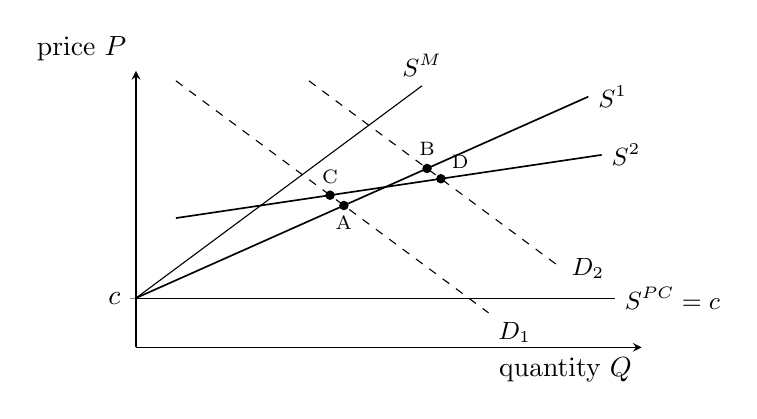
\begin{tikzpicture}
\begin{axis}[
  width=0.66\textwidth, height=0.42\textwidth,
  xmin=0, xmax=7.6, ymin=0, ymax=5.6,
  axis lines=left, xlabel={quantity $Q$}, ylabel={price $P$},
  xtick=\empty, ytick={1}, yticklabels={$c$},
  every axis x label/.style={at={(ticklabel* cs:1)}, anchor=north east},
  every axis y label/.style={at={(ticklabel* cs:1)}, anchor=south east},
  clip=false]
  \addplot[thin, domain=0:7.2, samples=2] {1} node[pos=1, right, font=\small] {$S^{PC} = c$};
  \addplot[thin, domain=0:4.3, samples=2] {1 + x} node[pos=1, above, font=\small] {$S^{M}$};
  \addplot[semithick, domain=0:6.8, samples=2] {1 + 0.6*x} node[pos=1, right, font=\small] {$S^{1}$};
  \addplot[semithick, domain=0.6:7.0, samples=2] {2.5 + 0.2*x} node[pos=1, right, font=\small] {$S^{2}$};
  \addplot[dashed, domain=0.6:5.3, samples=2] {6 - x} node[pos=1, below right, font=\small] {$D_1$};
  \addplot[dashed, domain=2.6:6.4, samples=2] {8 - x} node[pos=1, right, font=\small] {$D_2$};
  \addplot[only marks, mark=*, mark size=1.5pt] coordinates {(3.125,2.875) (4.375,3.625) (2.9167,3.0833) (4.5833,3.4167)};
  \node[below, font=\scriptsize] at (axis cs:3.125,2.85) {A};
  \node[above, font=\scriptsize] at (axis cs:4.375,3.68) {B};
  \node[above, font=\scriptsize] at (axis cs:2.9167,3.12) {C};
  \node[above right, font=\scriptsize] at (axis cs:4.6,3.42) {D};
\end{axis}
\end{tikzpicture}
\caption[Slope versus level of the supply relation]{Slope versus level of the supply relation. Inverse demand shifts from
$D_1\colon P = 6 - Q$ to $D_2\colon P = 8 - Q$, and marginal cost is $c = 1$. Industry 1 follows the conjectural-variations
supply relation $S^1\colon P = 1 + 0.6Q$ (points A and B). Industry 2 follows $S^2\colon P = 2.5 + 0.2Q$ (points C and D).
Both industries have average markup $2.25$ at average quantity $3.75$, an $m$-weighted average conduct of $0.6$. The conduct parameter
method estimates $0.6$ for industry 1 and $0.2$ for industry 2, and attributes the rest of industry 2's margin to a
marginal cost of $2.5$. $S^{PC}$ and $S^M$ are the competitive and monopoly supply relations. Drawn in the spirit of
Figure~1 of \citet{Corts1999}.}
\label{fig:03-corts-slope}
\end{figure}

The numbers in \cref{fig:03-corts-slope} are easy to check. On $S^1$, point A solves $6 - Q = 1 + 0.6Q$, so $Q = 3.125$
and the markup is $1.875$. Point B solves $8 - Q = 1 + 0.6Q$, so $Q = 4.375$ and the markup is $2.625$. On $S^2$, point C
solves $6 - Q = 2.5 + 0.2Q$, so $Q = 2.917$ and the markup is $2.083$. Point D gives $Q = 4.583$ and markup $2.417$. Both
pairs average a markup of $2.25$ at quantity $3.75$. The ratio $\frac{2.25}{3.75} = 0.6$ is the $m$-weighted average
conduct $\frac{\E[\theta_t m_t]}{\E[m_t]}$, since $m_t = Q_t$ when the slope of demand is $-1$.

\subsubsection{Corts's supergame model}

To show that the gap can be large in a coherent model, Corts studies efficient tacit collusion supported by repeated
interaction \citep[Section~3]{Corts1999}. The model is closely related to \citet{RotembergSaloner1986} when demand is
independent over time and to \citet{Kandori1991} when it is serially correlated \citep[fn.~2]{Corts1999}. We use
$\delta$ for the discount factor in the rest of this subsection. $N$
symmetric firms choose quantities every period. Inverse demand is $P_t = A(x_t) - BQ_t$ and marginal cost is $c(w_t)$,
where the demand state $x_t$ and the cost state $w_t$ are observed by all firms before they choose. A deviation is
punished by reversion to the one-shot Cournot equilibrium forever. An \emph{efficient} supergame equilibrium chooses, in
each state, the quantity that maximizes joint profit subject to the incentive constraint. Let $y_t = A(x_t) - c(w_t)$ be
the demand margin and $q$ the output of each firm.

The incentive constraint takes a simple form. A firm's collusive profit is $\pi(q) = q(y_t - BNq)$. Against rivals who
produce $(N - 1)q$, the best deviation produces $\frac{y_t - B(N - 1)q}{2B}$ and earns $\pi^b(q) = \frac{(y_t - B(N -
1)q)^2}{4B}$. The one-period gain from deviating is
\begin{align*}
\pi^b(q) - \pi(q) &= \frac{(y_t - B(N - 1)q)^2 - 4Bq(y_t - BNq)}{4B}\\
&= \frac{y_t^2 - 2B(N + 1)\, q\, y_t + B^2\left[(N - 1)^2 + 4N\right]q^2}{4B}\\
&= \frac{\left(y_t - B(N + 1)q\right)^2}{4B} .
\end{align*}
Let $\Lambda(x_t)$ be the expected discounted profit lost by entering the punishment phase \citep[eq.~15]{Corts1999}. It sums,
over future periods $i \ge 1$, $\delta^i$ times the expected excess of collusive over Cournot profit. The incentive
constraint is $\frac{(y_t - B(N + 1)q)^2}{4B} \le \Lambda(x_t)$. Collusive output lies below the Cournot output $q^c =
\frac{y_t}{B(N + 1)}$, so the constraint reads $y_t - B(N + 1)q \le 2\sqrt{B \Lambda(x_t)}$. The smallest sustainable output is
\begin{equation}\label{eq:03-corts-qtilde}
\tilde q_t = \frac{y_t}{B(N + 1)} - \frac{2\sqrt{B \Lambda(x_t)}}{B(N + 1)} \qquad \text{\citep[eq.~14]{Corts1999}}.
\end{equation}
The efficient output is the joint-monopoly output $q^m_t = \frac{y_t}{2BN}$ when it is sustainable, and $\tilde q_t$
otherwise. In industry units, conduct in state $t$ is $\theta_t = \frac{P_t - c_t}{BQ_t}$, which equals 1 at $q^m_t$ and
$\frac{1}{N}$ at $q^c$.

Equation \eqref{eq:03-corts-qtilde} shows why persistence matters. A higher demand state raises the gain from deviating,
which pushes output up toward Cournot. If demand is persistent, a higher state also raises expected future collusive
profits and so the cost of punishment $\Lambda(x_t)$, which pushes output down. When shocks are independent over time, only the
first effect operates. Then $\Lambda$ does not depend on $x_t$, and $\frac{\dd\tilde q_t}{\dd x_t} = \frac{A_1}{B(N + 1)}$, the
Cournot response.

\casehead{Simulation design and results}
Corts simulates a symmetric duopoly with linear demand and constant marginal cost. The demand and cost states each take
ten evenly spaced values. The cost state is independent over time, and its role is to identify demand. The demand state
follows a Markov chain that stays in the same state with probability $\varpi$ and moves to each other state with
probability $\frac{1 - \varpi}{9}$ (Corts calls this probability $\lambda$). Firms' quantities are computed by iterating
on $\Lambda(x_t)$ until convergence, and the conduct parameter method is applied to a sample from the resulting process.

\Cref{fig:03-corts-paper-fig2} reproduces Corts's results for positively correlated demand, in his firm-level
normalization (1 is Cournot and 2 is joint monopoly). He draws five lessons \citep[pp.~237--240]{Corts1999}. (a) For high
discount factors the method measures market power accurately whatever the demand process. (b) For low discount factors it
detects no market power when demand is independent over time. (c) It is accurate when demand is fully persistent. (d) It
becomes more accurate as demand becomes more persistent. (e) When demand states are negatively correlated, higher values
of the estimate go with lower values of the as-if parameter. The magnitudes are large. An estimate of 1.2 is consistent
with an as-if parameter of 1.3 when $\varpi = 0.9$ and of 1.9 when $\varpi = 0.5$ \citep[p.~238]{Corts1999}. Two
industries with similar estimates can thus differ greatly in collusiveness, and an industry whose demand becomes more or
less persistent can appear to change its conduct when it has not.

\begin{figure}[!htb]
\centering
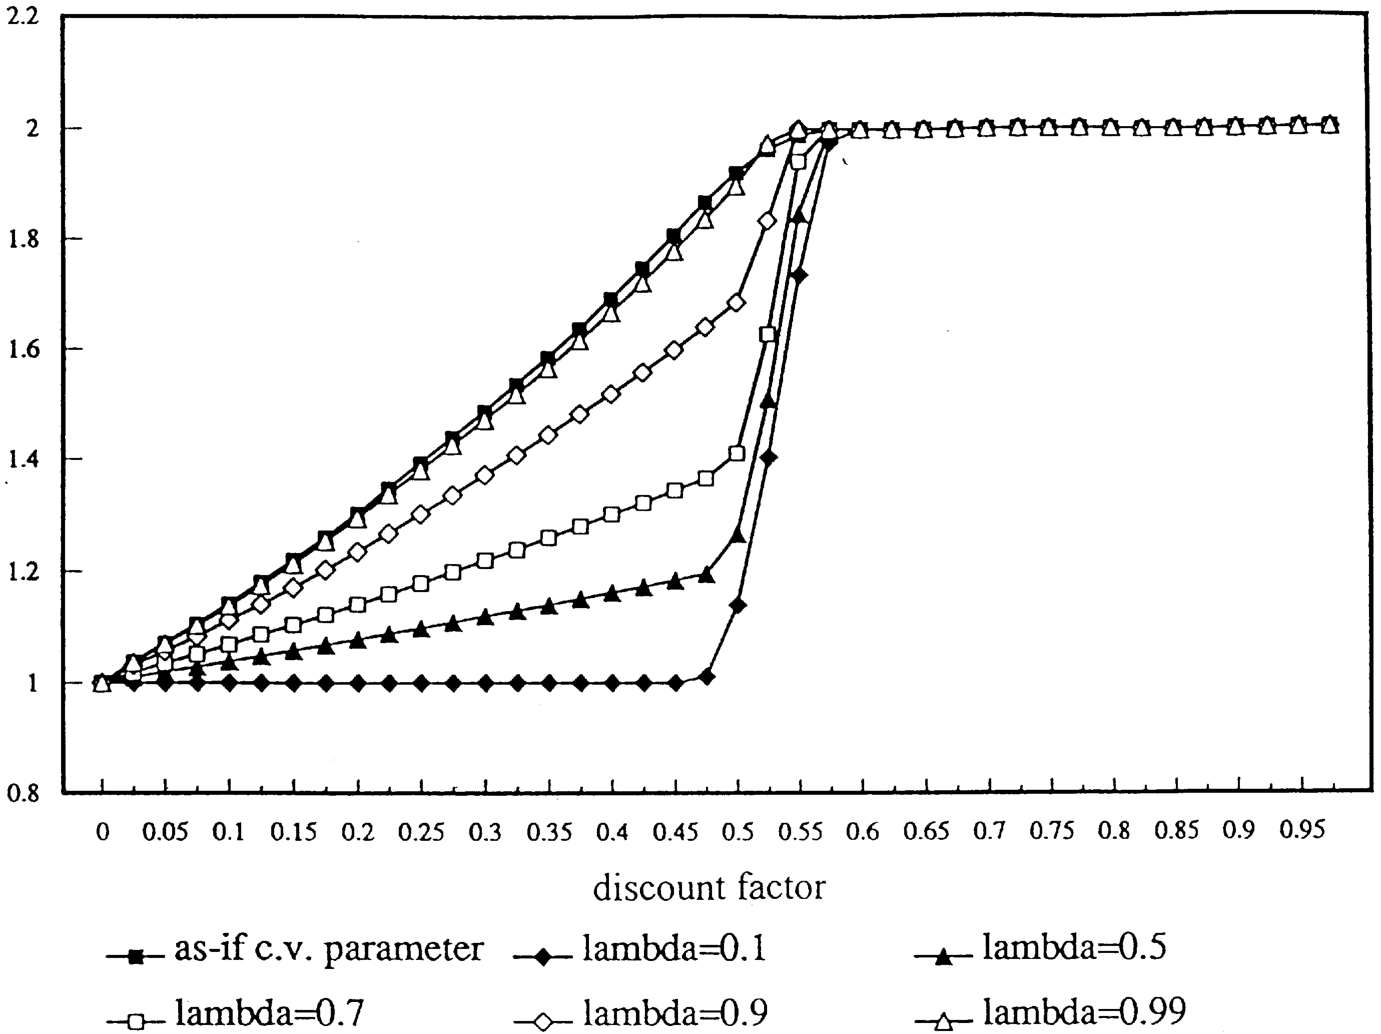
\includegraphics[width=0.85\textwidth]{figures/ch03/corts1999_fig2.png}
\caption[Conduct estimates in Corts's supergame simulations]{Conduct estimates in Corts's supergame simulations with
positively correlated demand, symmetric duopoly. The vertical axis is firm-level conduct (1 is Cournot, 2 is joint
monopoly). The top curve is the as-if conduct parameter. The other curves are conduct parameter estimates for demand
persistence $\varpi$ (``lambda'' in the original) of 0.1, 0.5, 0.7, 0.9 and 0.99. With ten states, $\varpi = 0.1$ makes
demand independent over time. Source: \citet{Corts1999},
Figure~2.}
\label{fig:03-corts-paper-fig2}
\end{figure}

Corts proves the main patterns \citep[Section~3.2]{Corts1999}. If joint monopoly is sustained in every state, the estimate
equals the as-if parameter (his Proposition~2). The monopoly supply relation is itself a conjectural-variations relation,
so it does not matter how monopoly is sustained. If demand is independent over time and monopoly is sustained in no state,
the estimate equals the Cournot value for every such discount factor (Proposition~3). Prices and profits rise with
$\delta$ over this range, yet the method detects none of the collusion. The proof is the one given above, since
$\frac{\dd\tilde q_t}{\dd x_t}$ equals the Cournot response. If demand is fully persistent, the estimate converges to the as-if
parameter (Proposition~4), because $\tilde q_t$ becomes proportional to the demand margin. If a higher demand state shifts
the distribution of future states to the right, the estimate exceeds the Cournot value whenever monopoly is sustained in no
state (Proposition~5). The method then detects some collusion but understates it. With negatively correlated demand, which
resembles seasonal variation, the estimate can fall below the Cournot value even though prices are above it. Corts warns
that seasonal dummies used as demand shifters may then fail to detect collusion, or produce estimates negatively correlated
with true conduct \citep[p.~240]{Corts1999}.

\subsubsection{A worked example: Bertrand collusion with demand shocks}\label{sec:03-corts-bertrand}

The following model is our own illustration, in the spirit of \citet{RotembergSaloner1986} and of Corts. It replaces
Cournot reversion with Bertrand reversion and delivers closed forms. $N$ symmetric firms sell a homogeneous good at constant
marginal cost $c$ and set prices every period. Demand is $Q_t = A_t - P_t$. The demand state $A_t$ is independent and
identically distributed over time with a continuous distribution on $[\underline A, \bar A]$, $\underline A > c$, and firms
observe it before pricing. Firms collude with grim-trigger strategies. Any deviation is followed by pricing at marginal cost
forever, which yields zero profit. Let $\Pi(p, A) = (p - c)(A - p)$ be industry profit and $\pi^m(A) = \frac{(A - c)^2}{4}$
monopoly profit.

\casehead{The incentive constraint}
Suppose firms charge $p \le p^m(A) = \frac{A + c}{2}$ and share the market equally. A deviator undercuts slightly, takes the
whole market and earns almost $\Pi(p, A)$ today and nothing afterward. Colluding yields $\frac{\Pi(p, A)}{N}$ today plus
$\frac{\delta}{1 - \delta}\frac{V}{N}$, where $V = \E[\Pi(p(A'), A')]$ is expected industry profit per period on the
collusive path. The incentive constraint is
\begin{equation*}
\Pi(p, A) - \frac{\Pi(p, A)}{N} \le \frac{\delta}{1 - \delta}\frac{V}{N}
\quad\Longleftrightarrow\quad
\Pi(p, A) \le K \equiv \frac{\delta V}{(1 - \delta)(N - 1)} .
\end{equation*}
Collusion thus caps industry profit at $K$ in every state. A price above $p^m(A)$ is never better. A deviator could then
undercut to $p^m(A)$ and earn $\pi^m(A)$, so the constraint would require $\pi^m(A) \le \frac{\Pi(p, A) + (N - 1)K}{N}$,
which fails whenever $\pi^m(A) > K$. The most profitable sustainable price is therefore
\begin{equation}\label{eq:03-bertrand-price}
p(A) =
\begin{cases}
\frac{A + c}{2} & \text{if } \pi^m(A) \le K ,\\[3pt]
\frac{A + c}{2} - \sqrt{\pi^m(A) - K} & \text{if } \pi^m(A) > K ,
\end{cases}
\end{equation}
where the second line is the lower root of $(p - c)(A - p) = K$. The cap binds in high-demand states, $A > A^* \equiv c +
2\sqrt K$. There the price falls as demand rises. Differentiating the second line,
$\frac{\dd p}{\dd A} = \frac{1}{2} - \frac{A - c}{4\sqrt{\pi^m(A) - K}} < 0$, because $\sqrt{\pi^m(A) - K} < \frac{A - c}{2}$.
These are the price wars during booms of \citet{RotembergSaloner1986}.

\casehead{The equilibrium cap}
Expected industry profit is $V = \E[\min\{\pi^m(A), K\}]$, so the cap solves the fixed-point equation
\begin{equation}\label{eq:03-bertrand-fixed}
K = \nu\, \E\left[\min\{\pi^m(A), K\}\right] \equiv T(K), \qquad \nu \equiv \frac{\delta}{(1 - \delta)(N - 1)} .
\end{equation}

\begin{lemma}[The most collusive equilibrium]\label{lem:03-fixed-point}
(i) If $\delta < 1 - \frac{1}{N}$, the only solution of \eqref{eq:03-bertrand-fixed} is $K = 0$, and firms price at cost.
(ii) If $\delta > 1 - \frac{1}{N}$, there is exactly one positive solution $K^*$. It is the largest fixed point, and the
iteration $K_{n+1} = T(K_n)$ started at any $K_0 \ge \nu\E[\pi^m(A)]$ decreases to $K^*$. (iii) Monopoly pricing in every
state is sustainable if and only if $\nu\,\E[\pi^m(A)] \ge \pi^m(\bar A)$.
\end{lemma}

\begin{proof}
The map $T$ is increasing and concave, because $\min\{\pi^m(A), K\}$ is increasing and concave in $K$ for every $A$. It
satisfies $T(0) = 0$, its right derivative at zero is $\nu$ (since $\pi^m(A) > 0$), and it is bounded by
$\nu\E[\pi^m(A)]$. The condition $\nu < 1$ is equivalent to $\delta < (1 - \delta)(N - 1)$, that is, to $\delta < 1 -
\frac{1}{N}$. (i) If $\nu < 1$, then $T(K) \le \nu K < K$ for every $K > 0$. (ii) If $\nu > 1$, the function
$T(K) - K$ is positive for small $K > 0$ and negative for large $K$, so it has a positive root. It is concave and equals
zero at $K = 0$ with positive slope there. A second positive root would force a concave function to be zero at two points
while positive between zero and the first, which is impossible. Starting at $K_0 \ge \nu\E[\pi^m(A)] \ge K^*$, the
sequence satisfies $K^* = T(K^*) \le T(K_n) \le K_n$, so it decreases and converges to a fixed point no smaller than
$K^*$, which must be $K^*$. (iii) If $K \ge \pi^m(\bar A)$, then $T(K) = \nu\E[\pi^m(A)]$, and the fixed point satisfies
$K \ge \pi^m(\bar A)$ exactly when $\nu\E[\pi^m(A)] \ge \pi^m(\bar A)$.
\end{proof}

Collusion above cost requires $\delta > 1 - \frac{1}{N}$, the familiar condition for Bertrand collusion with constant
demand. It plays the role of condition (i) in \citet{RotembergSaloner1986}, which requires that the number of firms not be
too large relative to the discount factor. They also select the greatest fixed point.
For any $\delta$ above it, the cap exceeds $\pi^m(\underline A)$. If $K \le \pi^m(\underline A)$, then $T(K) = \nu K >
K$, so no fixed point lies there. The lowest demand states are therefore always priced at the monopoly level.

\casehead{Conduct and the conduct parameter estimate}
The markup term is $m_t = Q_t$, because $\lvert\frac{\partial Q}{\partial P}\rvert = 1$. Conduct in state $A$ is
$\theta(A) = \frac{p(A) - c}{Q}$. In unconstrained states $p - c = Q = \frac{A - c}{2}$, so $\theta = 1$. In constrained
states $(p - c)Q = K$, so
\begin{equation*}
\theta(A) = \frac{K}{Q^2}, \qquad P - c = \frac{K}{Q} .
\end{equation*}
Conduct falls as demand rises, and the supply relation in the constrained region is a rectangular hyperbola. Its local
slope is $-\frac{K}{Q^2} = -\theta(A)$. Part (ii) of \cref{prop:03-corts} applies with $Z_t = A_t$, since $m_t = A_t - p(A_t)$
is increasing in $A_t$. The estimate is a weighted average of the local slope $+1$ in unconstrained states and $-\theta(A)$
in constrained states, so it can be negative while every $\theta(A)$ lies in $(0, 1]$.

\Cref{tab:03-corts-sim} and \cref{fig:03-corts-sim} report the numbers for $N = 2$, $c = 0$ and $A_t$ uniform on $[6, 10]$.
Population moments are computed by quadrature, and a regression on 200,000 simulated periods reproduces them to within
$0.002$. Collusion requires $\delta > 0.5$. Monopoly in every state requires $\nu\E[\pi^m(A)] \ge \pi^m(10)$, that is,
$\nu \ge \frac{25}{16.33}$, which holds for $\delta \ge 0.6048$. In between, the cap binds in the high-demand states. At
$\delta = 0.51$, conduct ranges from $0.17$ in the highest state to $1$ in the lowest, and its mean is $0.51$. The
$m$-weighted average conduct is $\frac{\E[P_t - c]}{\E[Q_t]} = \frac{2.34}{5.66} = 0.41$. The instrumental-variables
estimate is $-0.36$. A researcher would conclude that prices lie below the competitive level in an industry whose average
elasticity-adjusted Lerner index is about one half. The estimate turns positive only near $\delta = 0.56$ and catches up with
average conduct when monopoly is sustained everywhere. With $N = 3$ the pattern is the same: at $\delta = 0.677$ mean
conduct is $0.53$ and the estimate is $-0.36$.

\begin{table}[htbp]
\centering
\caption{Mean conduct and the conduct parameter estimate in the Bertrand supergame}
\label{tab:03-corts-sim}
\begin{threeparttable}
\begin{tabular}{@{}cccccc@{}}
\toprule
Discount factor & Profit cap & Cutoff state & Share of states & Mean conduct & IV estimate \\
$\delta$ & $K$ & $A^*$ & constrained & $\E[\theta_t]$ & $\hat\theta$ \\
\midrule
0.5001 & 9.30 & 6.10 & 0.98 & 0.28 & $-0.27$ \\
0.505 & 11.37 & 6.74 & 0.81 & 0.44 & $-0.35$ \\
0.51 & 12.54 & 7.08 & 0.73 & 0.51 & $-0.36$ \\
0.52 & 14.38 & 7.58 & 0.61 & 0.62 & $-0.33$ \\
0.53 & 15.94 & 7.99 & 0.50 & 0.71 & $-0.28$ \\
0.55 & 18.69 & 8.65 & 0.34 & 0.83 & $-0.10$ \\
0.57 & 21.15 & 9.20 & 0.20 & 0.92 & $0.21$ \\
0.6048 & 25.00 & 10.00 & 0.00 & 1.00 & $1.00$ \\
\bottomrule
\end{tabular}
\begin{tablenotes}[flushleft]\footnotesize
\item Notes: $N = 2$ Bertrand firms, marginal cost $c = 0$, demand $Q_t = A_t - P_t$ with $A_t$ independent and uniform on
$[6, 10]$, grim-trigger punishment at marginal cost. $K$ is the largest solution of \eqref{eq:03-bertrand-fixed}, and the
cap binds for $A_t > A^* = 2\sqrt K$. Conduct is $\theta_t = \frac{P_t - c}{Q_t}$, the elasticity-adjusted Lerner index.
The estimate is $\frac{\Cov(A_t, P_t - c)}{\Cov(A_t, Q_t)}$, the limit of the instrumental-variables estimator with a
constant and the demand state as instrument. For $\delta < 0.5$ prices equal cost and both measures are zero. Population
moments computed by quadrature.
\end{tablenotes}
\end{threeparttable}
\end{table}

\begin{figure}[htbp]
\centering
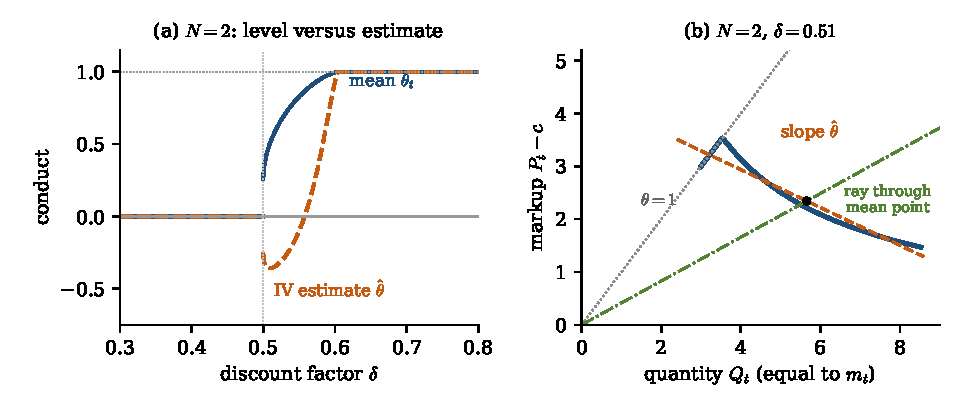
\includegraphics[width=\textwidth]{figures/ch03/corts_sim.pdf}
\caption[Level of conduct versus its estimate in a Bertrand supergame]{Level of conduct versus its estimate in a Bertrand
supergame with independent demand shocks ($N = 2$, $c = 0$, $A_t$ uniform on $[6, 10]$). Panel (a): mean conduct
$\E[\theta_t]$ and the instrumental-variables estimate $\hat\theta$ against the discount factor. Panel (b): the locus of
equilibrium markups and quantities at $\delta = 0.51$. It follows the monopoly ray $\theta = 1$ in low-demand states and the
hyperbola $P - c = \frac{K}{Q}$ in high-demand states. The dashed line through the mean point has slope $\hat\theta = -0.36$,
and the dash-dotted ray through the mean point has slope $0.41$, the $m$-weighted average conduct.}
\label{fig:03-corts-sim}
\end{figure}

The example and Corts's model reach the same conclusion by different routes. With Cournot reversion and independent
shocks, the estimate sticks at the Cournot value. With Bertrand reversion the static benchmark is price taking, and the
constant profit cap makes the constrained supply relation slope downward, so the estimate falls below zero. In both cases
the estimate reflects how the incentive constraint varies with demand, and it carries no direct information on the level
of conduct.

\subsubsection{Assessment}\label{sec:03-corts-assessment}

The critique changes how we read a conduct estimate. A constant-$\theta$ estimate measures the slope of the supply relation,
a weighted average of marginal responses of the markup to demand. Reading it as the level of conduct requires the marginal
and average relations to coincide. This holds in conjectural-variations models, under monopoly in every state, and in the
limit of fully persistent demand. Corts concludes that, when behavior results from efficient supergame collusion, the method
understates market power if demand shocks are not fully permanent. It may detect no market power at all when shocks are
transitory, even with average margins near the monopoly level \citep[pp.~244--245]{Corts1999}.

Three further points follow. First, the specification-test reading does not escape the critique. The estimate can equal
the Cournot value over a wide range of collusive equilibria. A failure to reject Cournot then carries little information,
and tests of the nested static models may lack power. Second, Corts argues that ``not even the positive correlation'' of
the estimate with the as-if parameter can be maintained across models \citep[p.~245]{Corts1999}. Comparisons of conduct
across industries or over time are therefore suspect. Third, the evidence available to Corts points the same way. In the
electricity study of \citet{Wolfram1999} and the sugar study of \citet{GenesoveMullin1998}, the estimates obtained without
cost data fall below the direct measures. Both studies were available to Corts as working papers. Corts notes that equality of the
two can be rejected in both cases \citep[p.~245]{Corts1999}. \Cref{sec:03-sugar,sec:03-electricity} examine both studies.

Genesove and Mullin frame the point in the same terms. The conduct parameter ``measures the marginal response of price, and
hence the markup, to changes in exogenous variables'' \citep[p.~2]{GenesoveMullin1995}. It therefore ``infers market power
from the marginal behavior of the markup, not from the level of the markup.'' They add an example
\citep[p.~3]{GenesoveMullin1995}. Supergame models such as \citet{RotembergSaloner1986} may make the marginal response of
price to demand shifters independent of the discount rate. It is then also independent of the price level at a baseline
state of demand.

The critique has limits. Corts's models are stylized, with linear demand, constant cost, perfect monitoring and an efficient
equilibrium, and the simulations are not calibrated to any industry. They show that the mismeasurement can be severe, and
they leave its size in a given application open. The direction of the bias depends on the persistence of demand, which the
researcher can sometimes measure.

The contribution is lasting. \citet[fn.~7]{BerryHaile2014} cite \citet{Corts1999} and \citet{ReissWolak2007} for the
fundamental problems of the conduct parameter approach. Corts calls for explicit structural models of conduct. The field
responded in three ways. It estimates dynamic models of collusion directly, as in the work on the railroad cartel of
\citet{Porter1983} and \citet{Ellison1994} (\cref{ch:collusion-evidence}). It tests a finite menu of conduct models within
richer demand systems (\cref{sec:03-other-routes}). And it validates the method where marginal cost is observed
(\cref{sec:03-sugar,sec:03-electricity}).

\subsection{Bounds instead of point estimates}\label{sec:03-bounds}

If conduct varies and a constant $\theta$ misleads, we can give up point identification. \citet[Section~2.2]{Rosen2007}
replaces the equilibrium assumption with known bounds on each firm's conduct in each period. The widest bounds are price
taking and monopoly. Conduct may vary freely within them, so the parameters of marginal cost are in general only set identified.
We present the idea in the homogeneous-good setting of this chapter.

Suppose only that industry conduct lies between price taking and joint monopoly, $\theta_t \in [0, 1]$, with no restriction
on how it varies across observations. The supply relation gives $P_t - mc_t = -\theta_t Q_t P'(Q_t)$. Since $-Q_tP'(Q_t)
\ge 0$, the bounds on $\theta_t$ imply $0 \le P_t - mc_t \le -Q_t P'(Q_t)$, that is,
\begin{equation}\label{eq:03-rosen-ineq}
P_t + Q_t P'(Q_t) \;\le\; mc_t \;\le\; P_t .
\end{equation}
Marginal cost lies between monopoly marginal revenue and price, observation by observation. With a parametric marginal
cost $mc_t = c(Q_t, W_t; \beta) + u^s_t$ and $\E[u^s_t \mid X_t] = 0$ for instruments $X_t$, the inequalities become
conditional moment inequalities:
\begin{equation*}
\E\left[P_t - c(Q_t, W_t; \beta) \mid X_t\right] \ge 0, \qquad
\E\left[c(Q_t, W_t; \beta) - P_t - Q_t P'(Q_t) \mid X_t\right] \ge 0 .
\end{equation*}
The \emph{identified set} is the set of $\beta$ that satisfy both for almost every $X_t$. Since $P'(Q_t)$ comes from an
estimated demand curve, estimation has two steps. Bounds on $\beta$ imply bounds on marginal cost, on markups and on each
$\theta_t$, without assuming that conduct is constant.

A deterministic example shows the geometry. Let $mc = b_0 + b_1 Q$ with true values $(b_0, b_1) = (2, 0.5)$, and let
inverse demand in market $t$ be $P = A_t - Q$. Four markets have $A_t = 8, 10, 12, 14$ and conduct $\theta_t = 0.2, 0.9,
0.5, 0.1$. The equilibrium solves $A_t - Q - (2 + 0.5Q) = \theta_t Q$, so $Q_t = \frac{A_t - 2}{1.5 + \theta_t}$. Each
market contributes the two half-planes $P_t - Q_t \le b_0 + b_1 Q_t \le P_t$ in the $(b_1, b_0)$ plane, and we add the
restrictions $b_0 \ge 0$ and $b_1 \ge 0$. \Cref{fig:03-rosen-bounds} shows the intersection. It is a quadrilateral with
$b_1 \in [0, 0.76]$ and $b_0 \in [0.80, 4.47]$. Without the sign restrictions the slope could range from $-1.38$ to $0.76$.
The implied bounds on conduct are informative in some markets. Conduct lies in $[0.66, 1]$ in the second market (true value
$0.9$) and in $[0.36, 0.73]$ in the third (true value $0.5$). In the first and fourth markets only the upper bound moves,
to $0.32$ and $0.42$ (true values $0.2$ and $0.1$).

\begin{figure}[htbp]
\centering
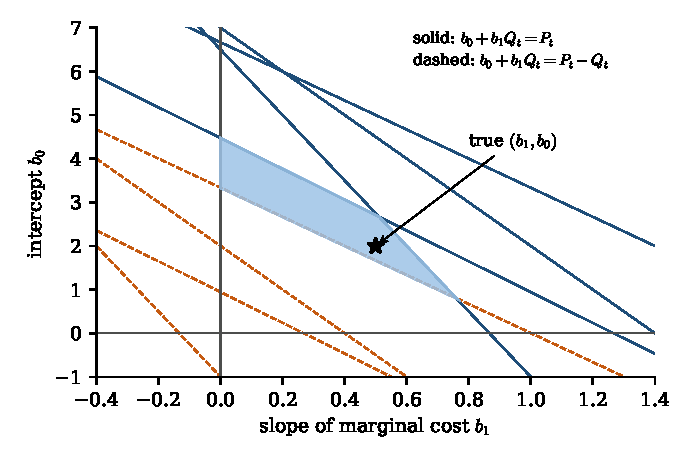
\includegraphics[width=0.60\textwidth]{figures/ch03/rosen_bounds.pdf}
\caption[Identified set for marginal cost when conduct varies freely]{Identified set for a linear marginal cost
$mc = b_0 + b_1 Q$ when conduct varies freely in $[0, 1]$. Each of four markets with inverse demand $P = A_t - Q$ restricts
$(b_1, b_0)$ to the band between a solid line (marginal cost equals price) and a dashed line (marginal cost equals monopoly
marginal revenue). The shaded region is the intersection with $b_0, b_1 \ge 0$. The star marks the true values $(0.5, 2)$.}
\label{fig:03-rosen-bounds}
\end{figure}

The set shrinks quickly when some markets sit near the extremes of conduct. Consider six markets with $A_t = 6, 8, \dots,
16$ and $\theta_t = 0.1, 0.8, 0.3, 1, 0, 0.6$, one of them competitive and one fully collusive. The identified set is then
a small triangle with $b_1 \in [0.33, 0.50]$ and $b_0 \in [2.00, 2.67]$. Every market's conduct is bounded within an
interval of width at most $0.1$. The approach trades precision for robustness. It needs no assumption on how conduct varies,
and it states plainly what the data cannot reveal. Its bounds can be wide, and inference requires methods for moment
inequalities. The Lerner bound \eqref{eq:03-lerner-bound} and Sullivan's bound in \cref{sec:03-sullivan} use the same
logic in reverse. A lower bound on marginal cost, the tax, bounds conduct from above.

\subsection{The record of conduct estimates}\label{sec:03-record}

Almost all estimates of conduct fall strictly between zero and one. The finding is unsurprising, yet it is useful against
extreme claims that an industry is perfectly competitive or fully cartelized. \Cref{tab:01-bresnahan-table} reproduces the
estimated Lerner indices that \citet[Table~17.1]{Bresnahan1989} collected from early studies. \Cref{sec:01-neio-lessons}
discusses the three conclusions he draws from them \citep[pp.~1052--1053]{Bresnahan1989}. He concludes that some
concentrated industries have high margins and that anticompetitive conduct is one cause. He also finds that the studies
reveal little about how market power relates to industry structure.

The entries of that table are margins, and they differ from conduct parameters by the factor $\varepsilon$. Bresnahan left
out studies whose estimates could not be converted into a Lerner index. These include the Panzar-Rosse and Sullivan
methods, which yield tests or bounds, and the residual demand method, whose elasticities equal the Lerner index only in
special cases \citep[fn.~47]{Bresnahan1989}. Two lessons of this section qualify the record further. A conduct estimate is
a slope, so estimates in $(0, 1)$ are compatible with conduct that swings between collusion and price wars
(\cref{sec:03-corts}). The most direct test of the methods compares them with observed costs, which is the task of
\cref{sec:03-sugar,sec:03-electricity}.
